\documentclass[justified]{tufte-book}

% ams
\usepackage{amssymb,amsmath}

\usepackage{ifxetex,ifluatex}
\usepackage{fixltx2e} % provides \textsubscript
\ifnum 0\ifxetex 1\fi\ifluatex 1\fi=0 % if pdftex
  \usepackage[T1]{fontenc}
  \usepackage[utf8]{inputenc}
\else % if luatex or xelatex
  \makeatletter
  \@ifpackageloaded{fontspec}{}{\usepackage{fontspec}}
  \makeatother
  \defaultfontfeatures{Ligatures=TeX,Scale=MatchLowercase}
  \makeatletter
  \@ifpackageloaded{soul}{
     \renewcommand\allcapsspacing[1]{{\addfontfeature{LetterSpace=15}#1}}
     \renewcommand\smallcapsspacing[1]{{\addfontfeature{LetterSpace=10}#1}}
   }{}
  \makeatother

\fi

% graphix
\usepackage{graphicx}
\setkeys{Gin}{width=\linewidth,totalheight=\textheight,keepaspectratio}

% booktabs
\usepackage{booktabs}

% url
\usepackage{url}

% hyperref
\usepackage{hyperref}

% units.
\usepackage{units}


\setcounter{secnumdepth}{2}

% citations


% pandoc syntax highlighting

% table with pandoc
\usepackage{longtable,booktabs,array}
\usepackage{calc} % for calculating minipage widths
% Correct order of tables after \paragraph or \subparagraph
\usepackage{etoolbox}
\makeatletter
\patchcmd\longtable{\par}{\if@noskipsec\mbox{}\fi\par}{}{}
\makeatother
% Allow footnotes in longtable head/foot
\IfFileExists{footnotehyper.sty}{\usepackage{footnotehyper}}{\usepackage{footnote}}
\makesavenoteenv{longtable}

% multiplecol
\usepackage{multicol}

% strikeout
\usepackage[normalem]{ulem}

% morefloats
\usepackage{morefloats}


% tightlist macro required by pandoc >= 1.14
\providecommand{\tightlist}{%
  \setlength{\itemsep}{0pt}\setlength{\parskip}{0pt}}

% title / author / date
\title{Odds \& Ends}
\author{Jonathan Weisberg}
\date{}

%\usepackage{MinionPro}
%\usepackage{fontspec}
%\newfontfamily\DejaSans{DejaVu Sans}

\newcommand{\given}{\mid}
\renewcommand{\neg}{\mathbin{\sim}}
\renewcommand{\wedge}{\mathbin{\&}}
\renewcommand{\u}{U}
\newcommand{\gt}{>}
\newcommand{\p}{Pr}
\newcommand{\E}{E}
\newcommand{\EU}{EU}
\newcommand{\pr}{Pr}
\newcommand{\po}{Pr^*}
\newcommand{\degr}{^{\circ}}
\definecolor{bookred}{RGB}{228,6,19}
\definecolor{bookblue}{RGB}{0,92,169}
\definecolor{bookpurple}{RGB}{114,49,94}

\newenvironment{epigraph}%
{
\begin{flushright}    
\begin{minipage}{20em}
\begin{flushright}
\itshape
}%
{
\end{flushright}
\end{minipage}
\end{flushright}
}
\newenvironment{problem}{\begin{quote}\normalsize}{\end{quote}}
\newenvironment{puzzle}{\begin{quote}\normalsize}{\end{quote}}
\def\argument{\list{}{\leftmargin3em}\item[]}
\let\endargument=\endlist 
\usepackage{fontawesome}
\newenvironment{warning}{\begin{itemize}\item[\faBan]}{\end{itemize}}
\usepackage{marvosym}
\newenvironment{info}{\begin{itemize}\item[\Info]}{\end{itemize}}

%%%% Kevin Godny's code for title page and contents from https://groups.google.com/forum/#!topic/tufte-latex/ujdzrktC1BQ
\makeatletter
\renewcommand{\maketitlepage}{%
\begingroup%
\setlength{\parindent}{0pt}
{\fontsize{18}{18}\selectfont\textit{\@author}\par}
\vspace{1.75in}{\fontsize{36}{14}\selectfont\@title\par}
\vspace{0.5in}{\fontsize{20}{14}\selectfont Introducing Probability \& Decision with a Visual Emphasis\par}
\vspace{0.5in}{\fontsize{14}{14}\selectfont\textsf{\smallcaps{v0.3 beta}}\par}
\vfill{\fontsize{14}{14}\selectfont\textit{An Open Access Publication}\par}
\thispagestyle{empty}
\endgroup
}
\makeatother

% Change shape from [display] to [block] to keep chapter numbers and titles on the same line
\titleformat{\chapter}%
  [block]% shape
  {\relax\ifthenelse{\NOT\boolean{@tufte@symmetric}}{\begin{fullwidth}}{}}% format applied to label+text
  {\itshape\huge\thechapter}% label
  {3em}% horizontal separation between label and title body
  {\huge\rmfamily\itshape}% before the title body
  [\ifthenelse{\NOT\boolean{@tufte@symmetric}}{\end{fullwidth}}{}]% after the title body


\usepackage{etoolbox}
% Jesse Rosenthal's code from https://groups.google.com/forum/#!topic/pandoc-discuss/wCF78X6SvwY
% Avoid new pagraph/indent after lists, quotes, etc.
\makeatletter
\newcommand{\gobblepars}{% 
    \@ifnextchar\par% 
        {\expandafter\gobblepars\@gobble}% 
        {}}
\newcommand{\eatpar}{\@ifnextchar\par{\@gobble}{}}
\newcommand{\forcepar}{\par}
\makeatother
\AfterEndEnvironment{quote}{\expandafter\gobblepars}
\AfterEndEnvironment{enumerate}{\expandafter\gobblepars}
\AfterEndEnvironment{itemize}{\expandafter\gobblepars}
\AfterEndEnvironment{description}{\expandafter\gobblepars}
\AfterEndEnvironment{example}{\expandafter\gobblepars}
\AfterEndEnvironment{argument}{\expandafter\gobblepars}
\AfterEndEnvironment{problem}{\expandafter\gobblepars}
\AfterEndEnvironment{info}{\expandafter\gobblepars}
\AfterEndEnvironment{warning}{\expandafter\gobblepars}
\AfterEndEnvironment{marginfigure}{\expandafter\gobblepars}
\AfterEndEnvironment{longtable}{\expandafter\gobblepars} % not working, why?
\makeatletter
\AfterEndEnvironment{longtable}{\par\@afterindentfalse\@afterheading} % this seems to work instead
\makeatother

\renewcommand*\descriptionlabel[1]{\hspace\labelsep\normalfont\em #1.}

% prevent extra space when \newthought follows \section
% see: https://tex.stackexchange.com/questions/291746/tufte-latex-newthought-after-section
\makeatletter
\def\tuftebreak{%
  \if@nobreak\else
    \par
    \ifdim\lastskip<\tufteskipamount
      \removelastskip \penalty -100
      \tufteskip
    \fi
  \fi
}
\makeatother

% indent lists a bit
\usepackage{enumitem}
\setlist[1]{leftmargin=24pt}

\def\labelitemii{$\circ$}

\begin{document}

\maketitle



{
\setcounter{tocdepth}{0}
\tableofcontents
}

\hypertarget{preface}{%
\chapter*{Preface}\label{preface}}
\addcontentsline{toc}{chapter}{Preface}

\newthought{This} textbook is awesome.

\begin{enumerate}
\def\labelenumi{\arabic{enumi}.}
\tightlist
\item
  It is open access, hence free.
\item
  It's also \href{https://github.com/jweisber/vip-source}{open source}, so other instructors can modify it to their liking.

  \begin{marginfigure}
   If you teach from this book I'd love to know: email or
   \href{https://twitter.com/jweisber}{tweet me}.
   \end{marginfigure}
\item
  It's available in both \href{http://jonathanweisberg.org/vip/_main.pdf}{PDF} and \href{http://jonathanweisberg.org/vip/}{HTML}. So it can be read comfortably on a range of devices, or printed.
\end{enumerate}

A ``cheat sheet'' summarizing key definitions and formulas appears in {[}Appendix{]}{[}Cheat Sheet{]} {[}A{]}{[}Cheat Sheet{]}. Further appendices cover the axiomatic construction of probability theory, Hume's problem of induction, and Goodman's new ridle of induction.

\newthought{I} usually get a mix of students in my course, with different ideological inclinations and varying levels of background. For some the technical material is easy, even review. For others, a healthy skepticism about scientific methods and discourses comes naturally. My goal is to get these students all more or less on the same page.

If it weren't for these tools, I never would have written this book. It wouldn't have been possible to create one that does all the things this book is meant to do. I also owe inspiration to Kieran Healy's book \href{http://socviz.co/}{\emph{Data Visualization: A Practical Introduction}}, which uses the same suite of tools. It gave me the idea to use those tools for an updated, open, and visually enhanced rendition of the classic material from Skyrms and Hacking.

Finally, I'm indebted to several teaching assistants and students who helped with earlier drafts. Thanks especially to Liang Zhou Koh and Meagan Phillips, who contributed several exercises; to Soroush Marouzi and Daniel Munro, who worked out the kinks during the first semester the book was piloted; and to the students in that course, who bore with us, and contributed several corrections of their own.

\hypertarget{part-part-i}{%
\part*{Part I}\label{part-part-i}}
\addcontentsline{toc}{part}{Part I}

\hypertarget{the-monty-hall-problem}{%
\chapter{The Monty Hall Problem}\label{the-monty-hall-problem}}

\begin{epigraph}
When tackling a math problem,\\
I encourage students to draw a picture.\\
---Francis Su
\end{epigraph}

\newthought{Imagine} you're on a game show. There are three doors, one with a prize behind it. You're allowed to pick any door, so you choose the first one at random, door A.

\begin{marginfigure}
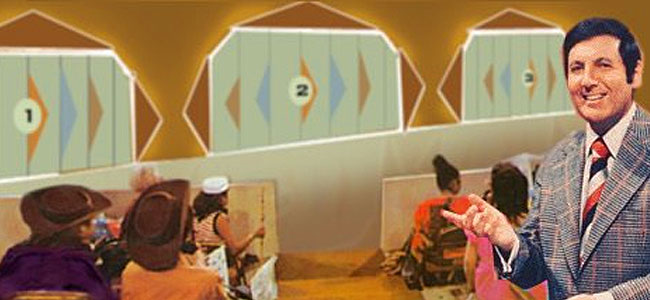
\includegraphics{img/lets_make_a_deal.png} Monty Hall was creator and
host of the game show \emph{Let's Make a Deal}.
\end{marginfigure}

Now the rules of the game require the host to open one of the other doors and let you switch your choice if you want. Because the host doesn't want to give away the game, they always open an empty door.

In your case, the host opens door C: no prize, as expected. ``Do you want to switch to door B?'' the host asks.

Pause a moment to think about your answer before reading on.

\newthought{What} did you decide? Did you conclude it doesn't matter whether you stick with door A or switch to door B?

\begin{marginfigure}
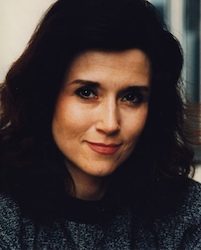
\includegraphics{img/marilyn_vos_savant.png} Marilyn vos Savant made the
Monty Hall problem famous when she solved it correctly in her magazine
column. Read about it
\href{https://www.nytimes.com/1991/07/21/us/behind-monty-hall-s-doors-puzzle-debate-and-answer.html}{here}.
\end{marginfigure}

If so, you're in good company. Most people find this answer sensible, including some professors of statistics and mathematics. They figure there are only two possibilities remaining, door A and door B, each with the same one-in-two chance of being the winner. So it doesn't matter which one you pick.

But the right answer is you should switch. Door B is now twice as likely to be the winner as door A. Why?

The reason is subtle. One way to think about it is that the host's choice of which door to open is a bit of a tell. Maybe they \emph{had} to open door C, because the prize is behind door B and they didn't want to give that away. Of course, it could be behind door A instead, so maybe they just picked door C at random. But there was only a one-in-three chance the prize would be behind door A. Which means there's a two-in-three chance they didn't really have a choice, they had to open door C to avoid showing you the prize behind door B.

\begin{marginfigure}
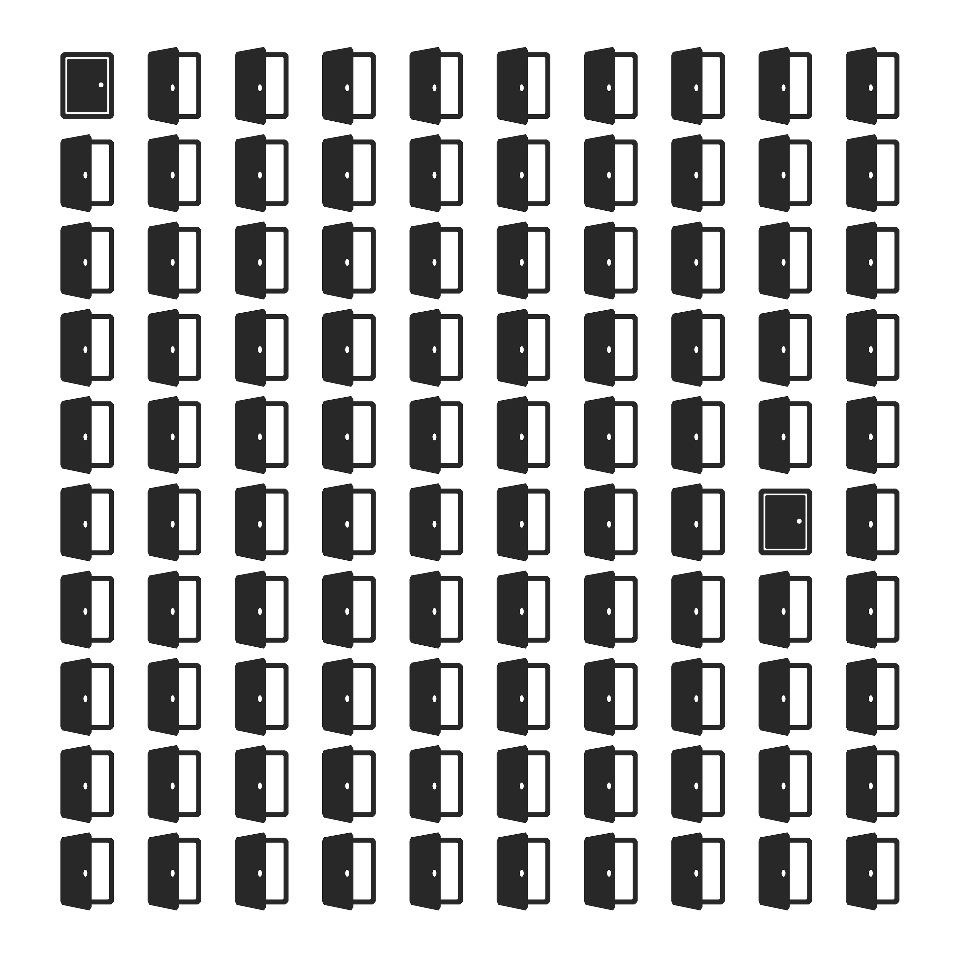
\includegraphics{_main_files/figure-latex/montygrid-1} \caption[The hundred-door version of the Monty Hall problem, suggested by Marilyn vos Savant]{The hundred-door version of the Monty Hall problem, suggested by Marilyn vos Savant}\label{fig:montygrid}
\end{marginfigure}

Here's another way to think about it. Imagine the game had a hundred doors instead of just three. And suppose again you start by picking the first door at random. Then the host opens \emph{all the other doors but one}, door \(59\) let's say. You have to ask yourself: why did they pick door \(59\) to leave closed?? Almost certainly because that's where the prize is hidden! Maybe you got really lucky and picked right with the first door at the beginning. But it's way more likely you didn't, and the host had to keep door \(59\) closed to avoid giving away the game.

\hypertarget{diagramming-the-solution}{%
\section{Diagramming the Solution}\label{diagramming-the-solution}}

\begin{marginfigure}
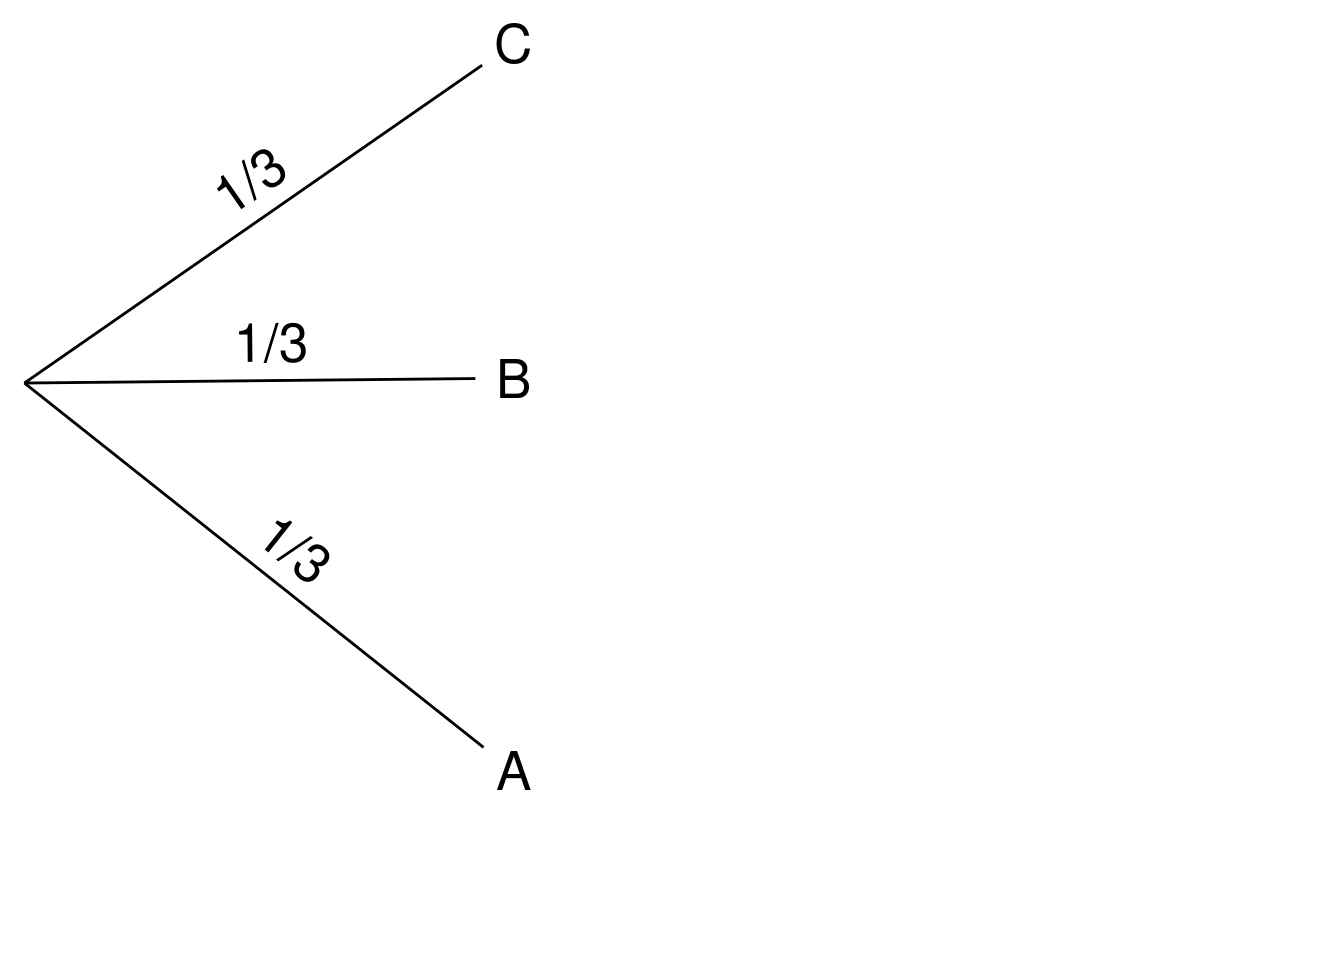
\includegraphics{_main_files/figure-latex/montytree1-1} \caption[First stage of a tree diagram for the Monty Hall problem]{First stage of a tree diagram for the Monty Hall problem}\label{fig:montytree1}
\end{marginfigure}
\begin{marginfigure}
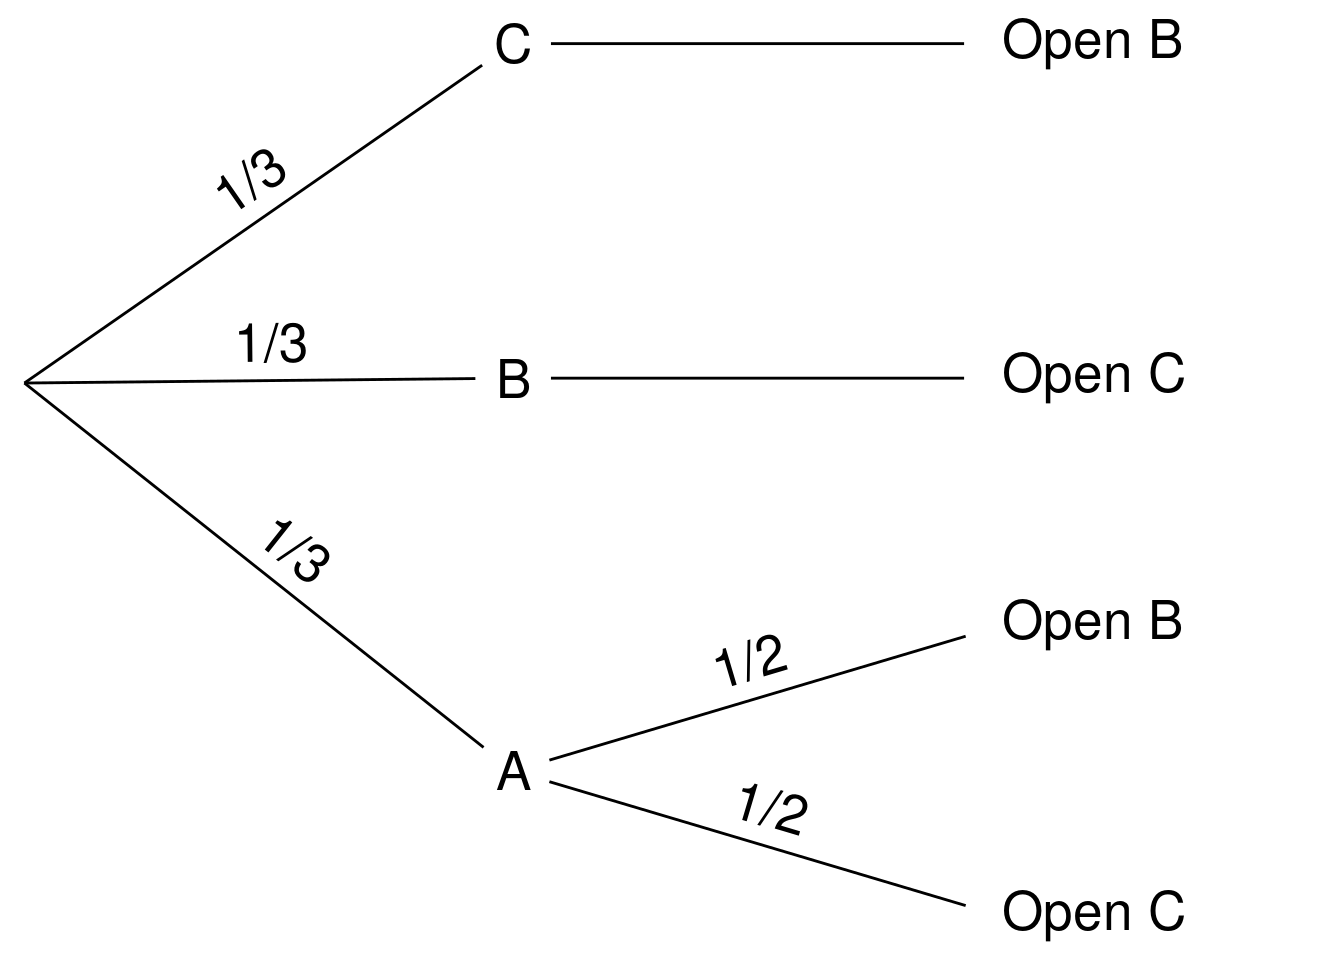
\includegraphics{_main_files/figure-latex/montytree2-1} \caption[Second stage]{Second stage}\label{fig:montytree2}
\end{marginfigure}
\begin{marginfigure}
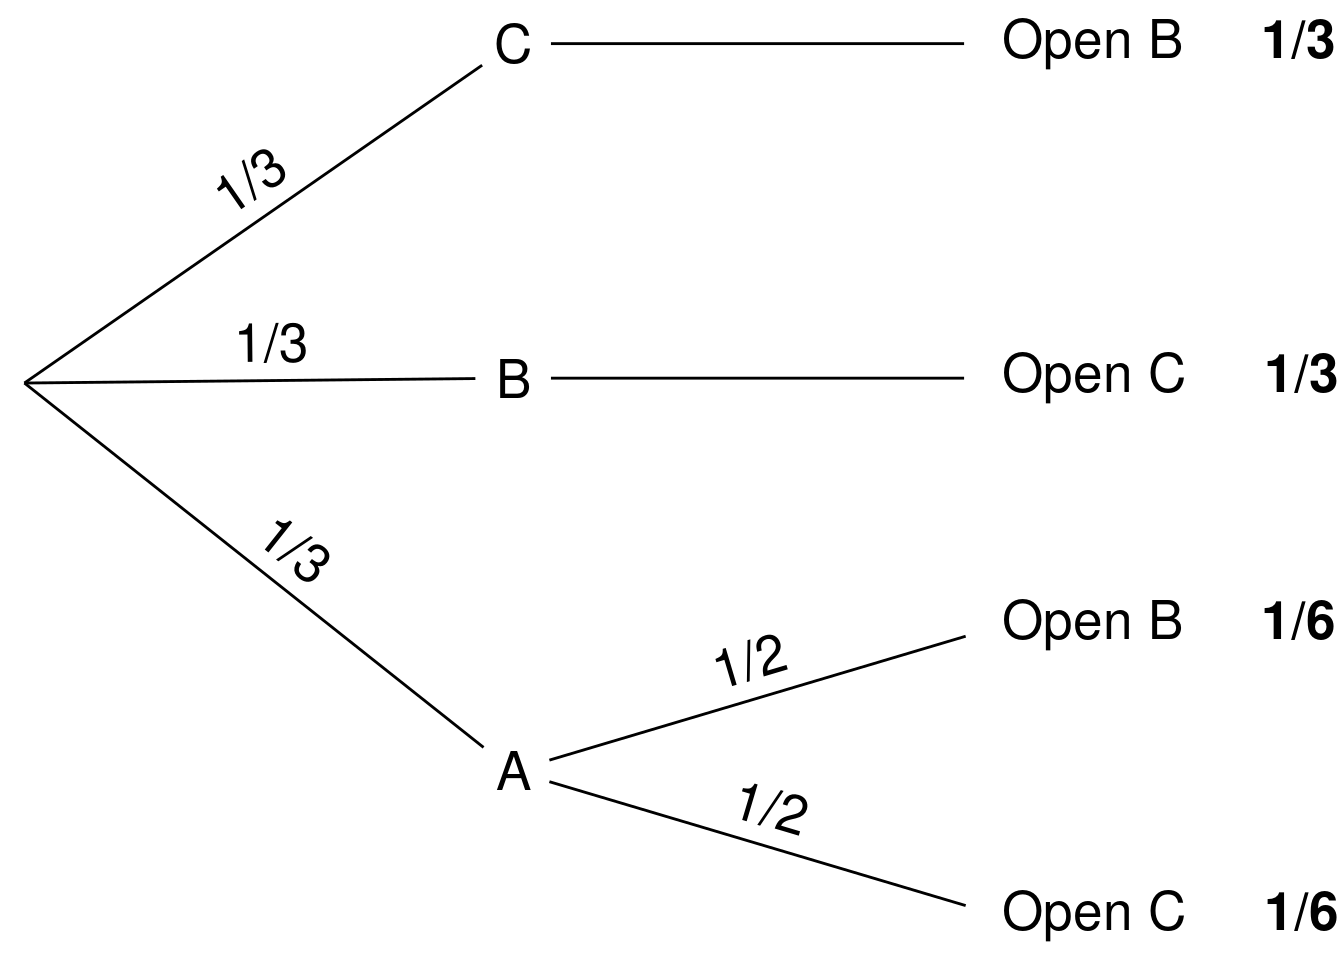
\includegraphics{_main_files/figure-latex/montytree3-1} \caption[Third and final stage]{Third and final stage}\label{fig:montytree3}
\end{marginfigure}

A picture helps clarify things. At first the prize could be behind any of the three doors, with equal probability each way. So we draw a tree with three branches, each labeled with a probability of \(1/3\). Figure \ref{fig:montytree1} shows the result.

Now, which door the host opens may depend on where the prize is, i.e.~which branch we're on. If it's behind door C, they won't show you by opening that door. They would have to open door B in this case.

Likewise, if the prize is behind door B, then opening door C is their only option.

Only if the prize is behind door A do they have a choice: open either door B or door C. In that case it's a tossup which door they'll open, so each of those possibilities has a 1/2 chance. Check out Figure \ref{fig:montytree2}.

Now imagine playing the game over and over. A third of the time things will follow the top path; a third of the time they'll follow the middle one; and the remaining third they'll follow one of the two bottom paths.

When things follow the bottom branches, half of those times the host will open door B, and half the time they'll open door C. So one in every six plays will follow the \emph{A-and-Open-B} path. And one in every six plays will follow the \emph{A-and-Open-C} path. See Figure \ref{fig:montytree3}.

Now we can understand what happens when the host opens door C. Usually it's because the prize is behind door B. Sometimes they open door C because the prize is behind door A instead. But that's only a sixth of the time, compared to a third of the time where they open door C because the prize is behind door B.

So when you see the host open door C, you should think it's more likely you're on the middle branch, with the prize behind door B. Switch!

\hypertarget{lessons}{%
\section{Lessons Learned}\label{lessons}}

Tree diagrams are a handy tool for solving probability problems. They also illustrate some central concepts of probability.

Probabilities are numbers assigned to possibilities. In the Monty Hall problem, there are three possibilities for where the prize is: door A, door B, and door C. Each of these possibilities starts with the same probability: 1/3.

Some possibilities are \textbf{\emph{mutually exclusive}}, meaning only one of them can obtain. The prize can't be behind door A and door B, for example. Here are more examples of mutually exclusive possibilities:

\begin{itemize}
\tightlist
\item
  A coin can land heads or tails, but it can't do both on the same toss.
\item
  A card drawn from a standard deck could be either an ace or a queen, but it can't be both.
\item
  The temperature at noon tomorrow could be 20 degrees, or it could be 25 degrees, but it can't be both.
\end{itemize}

When possibilities are mutually exclusive, their probabilities add up. For example, the initial probability the prize will be behind either door A or door B is \(1/3 + 1/3 = 2/3\). And the probability a card drawn from a standard deck will be either an ace or a queen is \(4/52 + 4/52 = 8/52 = 2/13\).

Another key concept is possibilities that are \textbf{\emph{exhaustive}}. In the Monty Hall problem, the prize has to be behind one of the three doors, so A, B, and C ``exhaust'' all the possibilities. Here are more examples of exhaustive possibilities:

\begin{itemize}
\tightlist
\item
  A card drawn from a standard deck must be either red or black.
\item
  The temperature at noon tomorrow must be either above zero, below zero, or zero.
\end{itemize}

\begin{marginfigure}
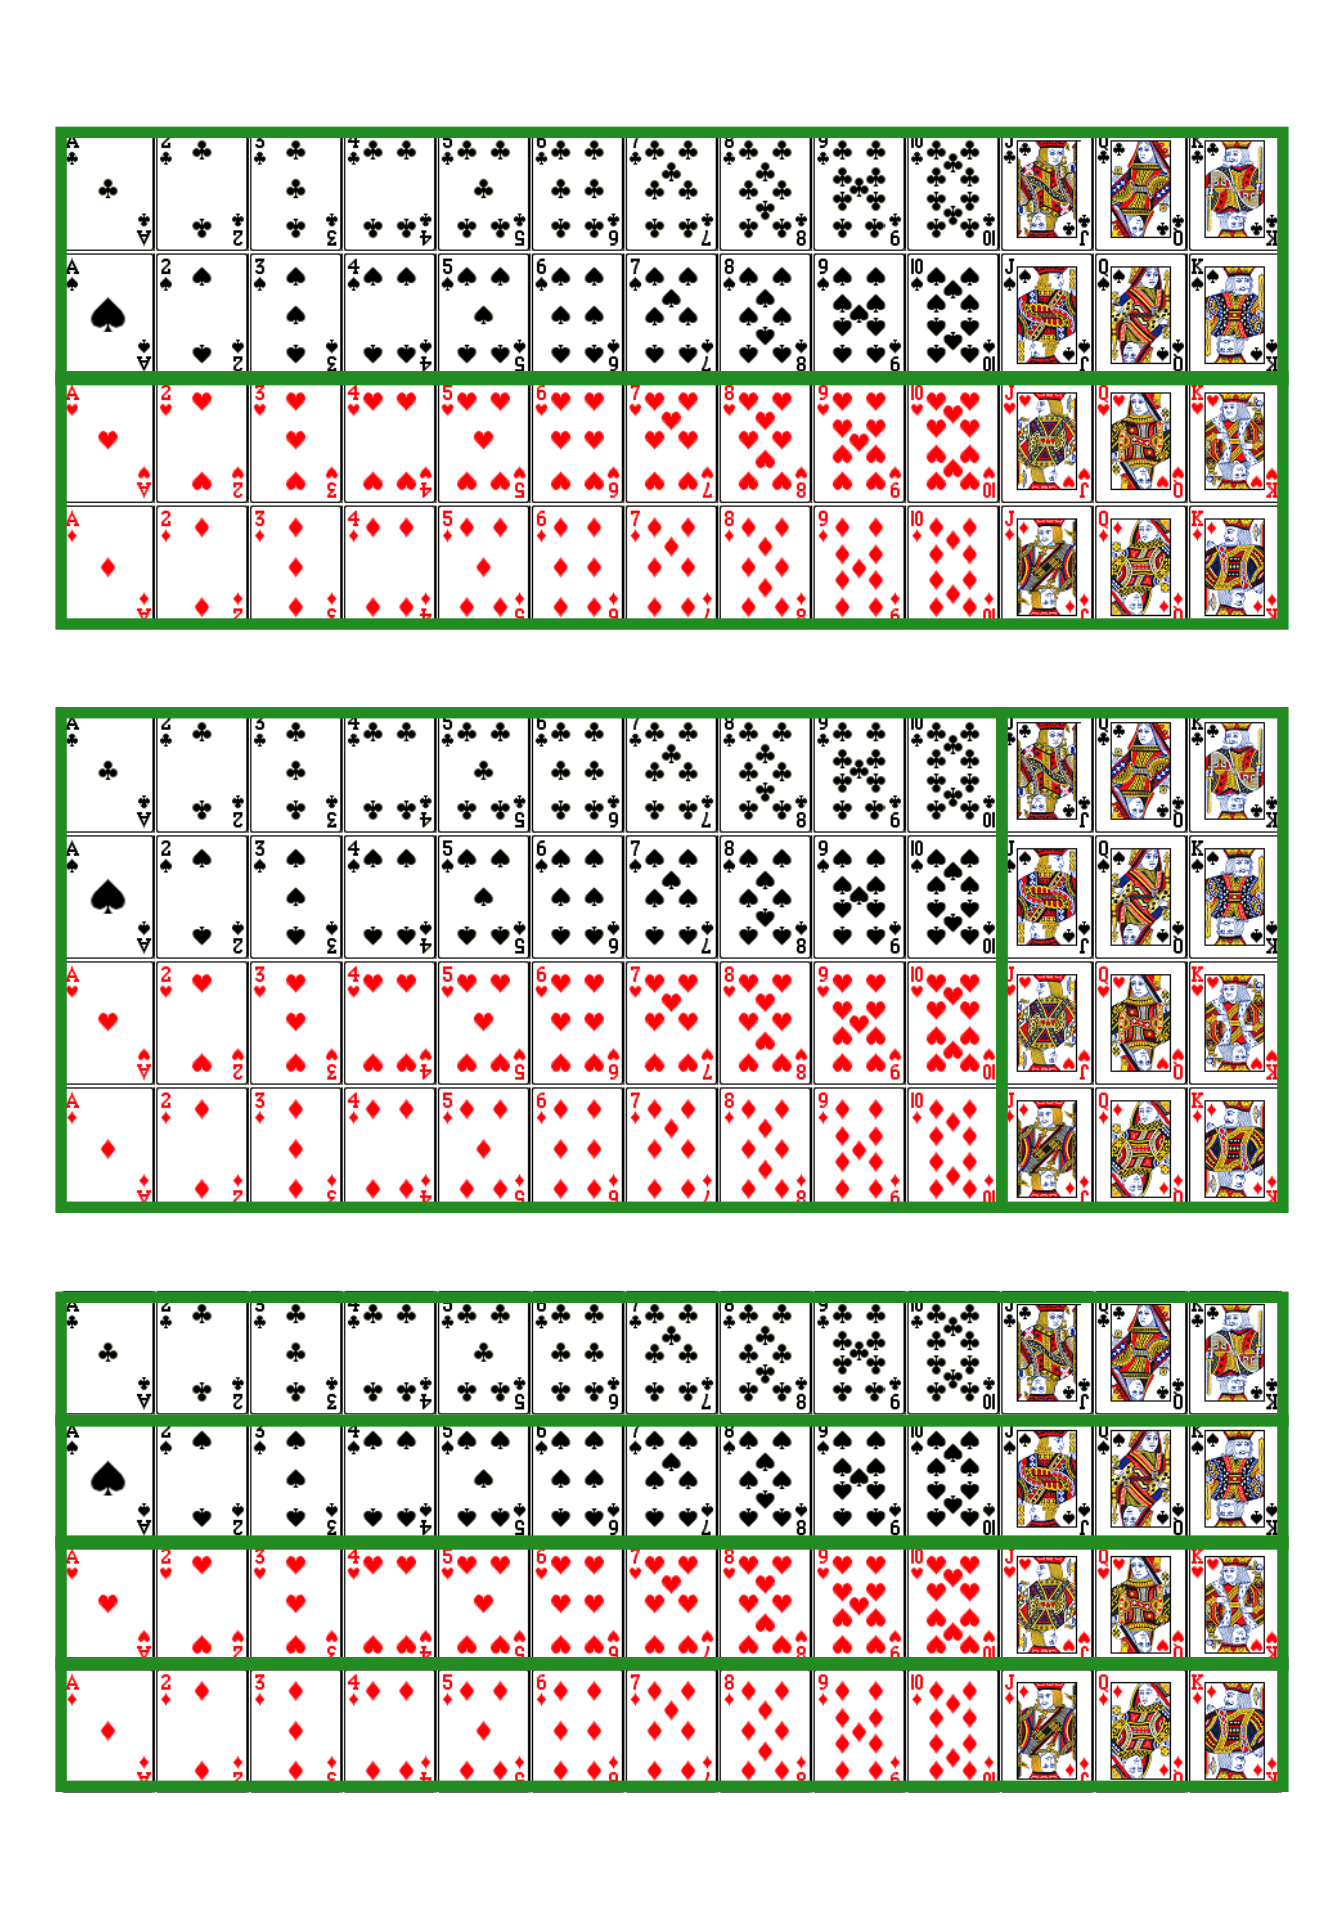
\includegraphics{_main_files/figure-latex/unnamed-chunk-5-1} \caption[Three  partitions for a card drawn from a standard deck]{Three  partitions for a card drawn from a standard deck}\label{fig:unnamed-chunk-5}
\end{marginfigure}

\newthought{In our} tree diagrams, each branch-point always uses a set of possibilities that is \emph{both} exclusive \emph{and} exhaustive. The first split on the three doors covers all the possibilities for where the prize might be, and only one of those possibilities can be the actual location of the prize. Likewise for the second stage of the diagram. On the bottom branch for example, the host must open either door B or door C given the rules, but he will only open one or the other.

When a set of possibilities is both exclusive and exhaustive, it's called a \textbf{\emph{partition}}. A partition ``carves up'' the space of possibilities into distinct, non-overlapping units.

There can be more than one way to partition the space of possibilities. For example, a randomly drawn playing card could be black or red; it could be a face card or not; and it could be any of the four suits (\(\heartsuit\), \(\diamondsuit\), \(\clubsuit\), \(\spadesuit\)).

When possibilities form a partition, their probabilities must add up to 1. Initially, the probability the prize will be behind one of the three doors is \(1/3 + 1/3 + 1/3 = 1\). And the probability that a card drawn from a standard deck at random will be either red or black is \(1/2 + 1/2 = 1\).

In a way, the fundamental principle of probability is that probabilities over a partition must add up to 1.

\newthought{Tree} diagrams follow a few simple rules based on these concepts. The parts of a tree are called \emph{nodes}, \emph{branches}, and \emph{leaves}: see Figure \ref{fig:treeparts}.

\begin{figure}
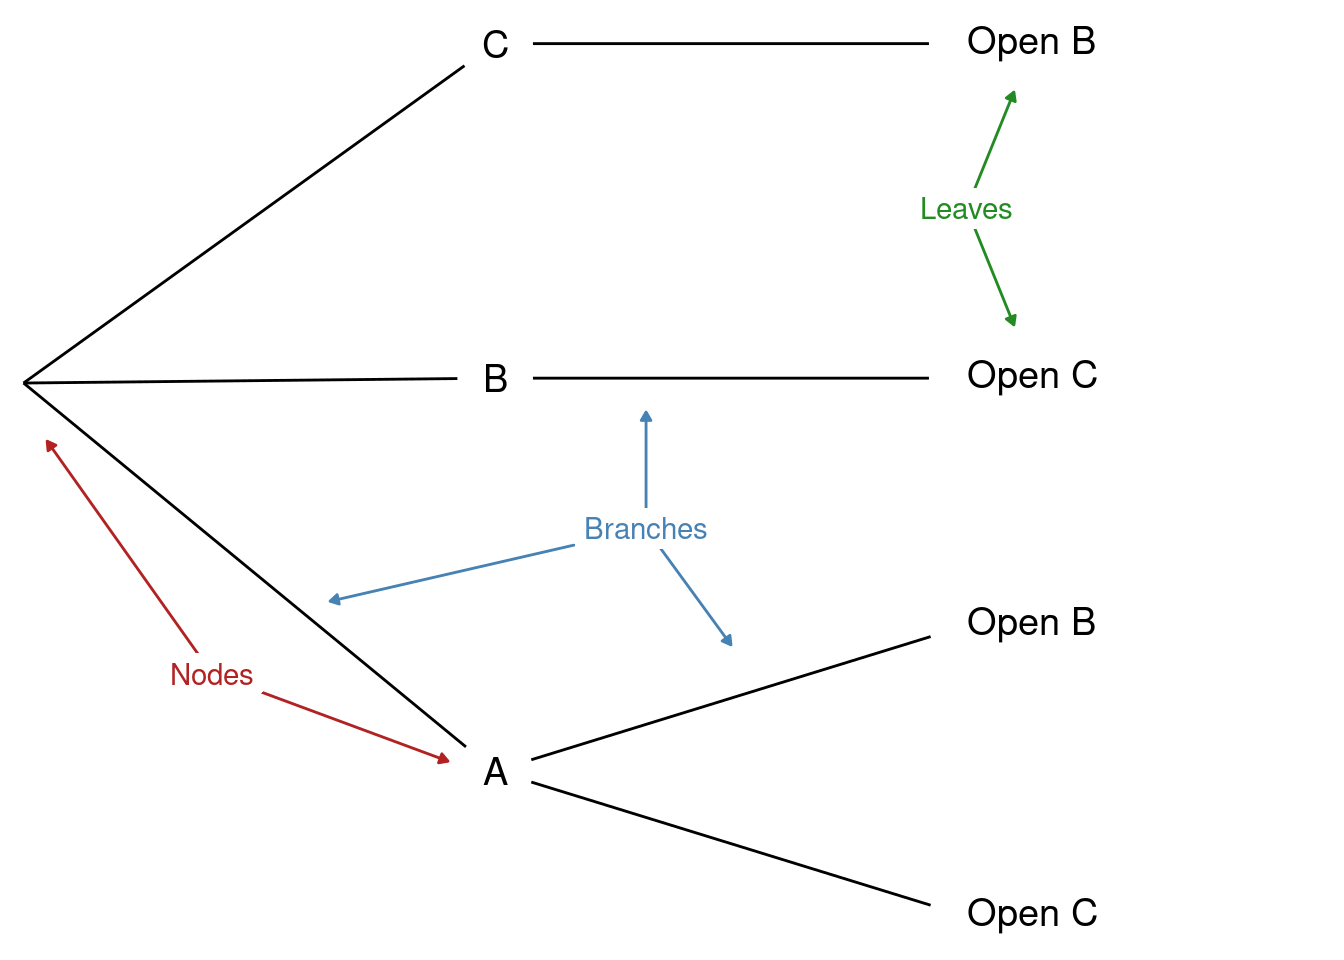
\includegraphics{_main_files/figure-latex/treeparts-1} \caption[The parts of a tree diagram]{The parts of a tree diagram: nodes, branches, and leaves}\label{fig:treeparts}
\end{figure}

The rules for a tree are as follows.

\begin{itemize}
\item
  \emph{Rule 1.} Each node must branch into a partition. The subpossibilities that emerge from a node must be mutually exclusive, and they must include every way the possibility from which they emerge could obtain.
\item
  \emph{Rule 2.} The probabilities emerging from a node must add to \(1\). If we add up the numbers on the branches immediately coming out of a node, they should add to \(1\).
\item
  \emph{Rule 3.} The probability on a branch is \emph{conditional} on the branches leading up to it. Consider the bottom path in the Monty Hall problem. The probability the host will open door C is \(1/2\) there because we're assuming the prize is behind door A.
\item
  \emph{Rule 4.} The probability of a leaf is calculated by multiplying across the branches on the path leading to it. This number represents the probability that all possibilities on that path occur.
\end{itemize}

Notice, Rule 4 is how we got the final probabilities we used to solve the Monty Hall problem (the numbers in bold).

\hypertarget{exercises}{%
\section*{Exercises}\label{exercises}}
\addcontentsline{toc}{section}{Exercises}

\begin{enumerate}
\item
  True or false: in the Monty Hall problem, it's essential to the puzzle that the host doesn't want to expose the prize. If they didn't care about giving away the location of the prize, there would be no reason to switch when they open door C.
\item
  In the version of the Monty Hall problem with a hundred doors, after the host opens every door except door 1 (your door) and door 59, the chance the prize is behind door 59 is:

  \begin{enumerate}
  \def\labelenumii{\alph{enumii}.}
  \tightlist
  \item
    1/100
  \item
    1/99
  \item
    1/2
  \item
    99/100
  \end{enumerate}
\item
  Imagine three prisoners, A, B, and C, are condemned to die in the morning. But the king decides to pardon one of them first. He makes his choice at random and communicates it to the guard, who is sworn to secrecy. She can only tell the prisoners that one of them will be released at dawn, she can't say who.

  Prisoner A welcomes the news, as he now has a \(1/3\) chance of survival. Hoping to go even further, he says to the guard, ``I know you can't tell me whether I am condemned or pardoned. But at least one other prisoner must still be condemned, so can you just name one who is?''. The guard tells him that B is still condemned. ``Ok,'' says A, ``then it's either me or C who was pardoned. So my chance of survival has gone up to 1/2.''

  Is prisoner A's reasoning correct? Use a probability tree to explain why/why not.
\item
  In a probability tree, each branch point should split into possibilities that are:

  \begin{enumerate}
  \def\labelenumii{\alph{enumii}.}
  \tightlist
  \item
    Mutually exclusive.
  \item
    Exhaustive.
  \item
    Both mutually exclusive and exhaustive.
  \item
    None of the above.
  \end{enumerate}
\item
  Suppose you have two urns. The first has two black marbles and two white marbles. The second has three black marbles and one white marble. You are going to flip a fair coin to select one of the urns at random, and then draw one marble at random. What is the chance you will select a black marble?

  Hint: draw a probability tree and ask yourself, ``if I did this experiment over and over again, how often would I draw a black marble in the long run?''

  \begin{enumerate}
  \def\labelenumii{\alph{enumii}.}
  \tightlist
  \item
    5/8
  \item
    3/8
  \item
    1/2
  \item
    1/4
  \end{enumerate}
\item
  An ice cream counter sells 4 different flavours of ice cream (chocolate, vanilla, strawberry, mint). There are \(2\) toppings (fudge, caramel), and \(3\) kinds of sprinkles (chocolate, rainbow, purple). You order by picking a flavour, a topping, and a kind of sprinkles.

  \begin{enumerate}
  \def\labelenumii{\alph{enumii}.}
  \tightlist
  \item
    How many possible orders are there?
  \item
    If you make your three choices randomly, what is the probability your order will have strawberry ice cream but not rainbow sprinkles?
  \end{enumerate}
\end{enumerate}

\hypertarget{the-problem-of-induction}{%
\chapter{The Problem of Induction}\label{the-problem-of-induction}}

\begin{epigraph}
It's tough to make predictions, especially about the future.\\
---Yogi Berra
\end{epigraph}

\newthought{Many} inductive arguments work by projecting an observed pattern onto as-yet unobserved instances. All the ravens we've observed have been black, so all ravens are. All the emeralds we've seen have been green, so all emeralds are.

The assumption that the unobserved will resemble the observed seems to be central to induction. Philosophers call this assumption the \emph{Principle of Induction}.\footnote{See \protect\hyperlink{indargs}{Section} \ref{indargs} and \protect\hyperlink{grue}{Appendix} \ref{grue} for previous discussions of the Principle of Induction.} But what justfies this assumption? Do we have any reason to think the parts of reality we've observed so far are a good representation of the parts we haven't seen yet?

Actually there are strong reasons to doubt whether this assumption can be justified. It may be impossible to give any good argument for expecting the unobserved to resemble the observed.

\hypertarget{the-dilemma}{%
\section*{The Dilemma}\label{the-dilemma}}
\addcontentsline{toc}{section}{The Dilemma}

We noted in {[}Chapter 2{]}{[}Logic{]} that there are two kinds of argument, inductive and deductive. Some arguments establish their conclusions necessarily, others only support them with high probability. If there is an argument for the Principle of Induction, it must be one of these two kinds. Let's consider each in turn.

Could we give an inductive argument for the Principle of Induction? At first it seems we could. Scientists have been using inductive reasoning for millenia, often with great success. Indeed, it seems humans, and other creatures too, have relied on it for much longer, and could not have survived without it. So the Principle of Induction has a very strong track record. Isn't that a good argument for believing it's correct?

\begin{marginfigure}
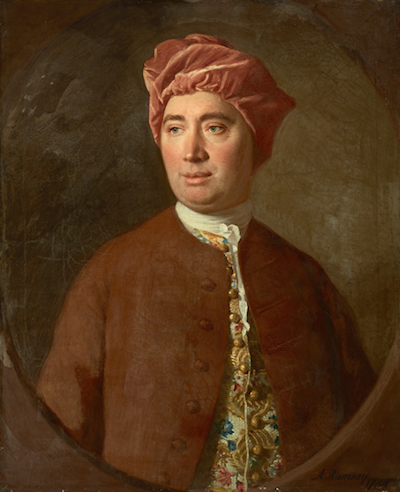
\includegraphics[width=1.33in]{img/hume} \caption[David Hume (1711--1776) raised the problem of induction in $1739$]{David Hume (1711--1776) raised the problem of induction in $1739$. Our presentation of it here is somewhat modernized from his original argument.}\label{fig:unnamed-chunk-7}
\end{marginfigure}

No, because the argument is circular. It uses the Principle of Induction to justify believing in the Principle of Induction. Consider that the argument we are attempting looks like this:

\begin{argument}
The principle has worked well when we've used it in the past.\\
Therefore it will work well in future instances.
\end{argument}

This is an inductive argument, an argument from observed instances to ones as yet unobserved. So, under the hood, it appeals to the Principle of Induction. But that's exactly the conclusion we're trying to establish. And one can't use a principle to justify itself.

What about our second option: could a deductive argument establish the Principle of Induction? Well, by definition, a deductive argument establishes its conclusion with necessity. Is it necessary that the unobserved will be like the observed? It doesn't look like it. It seems perfectly possible that tomorrow the world will go haywire, randomly switching from pattern to pattern, or even to no pattern at all.

Maybe tomorrow the sun will fail to rise. Maybe gravity will push apart instead of pull together, and all the other laws of physics will reverse too. And just as soon as we get used to those patterns and start expecting them to continue, another pattern will arise. And then another. And then, just as we give up and come to have no expectation at all about what will come next, everything will return to normal. Until we get comfortable and everything changes again.

Thankfully, our universe hasn't been so mischievous. We get surprised now and again, but for the most part inductive reasoning is pretty reliable, when we do it carefully. But we're lucky in this respect, is the point.

Nature \emph{could} have been mischievous, totally unpredictable. It is not a necessary truth that the unobserved must resemble the observed. And so it seems there cannot be a deductive argument for the Principle of Induction. Because such an argument would establish the principle as a necessary truth.

\hypertarget{the-problem-of-induction-vs.-the-grue-paradox}{%
\section*{The Problem of Induction vs.~the Grue Paradox}\label{the-problem-of-induction-vs.-the-grue-paradox}}
\addcontentsline{toc}{section}{The Problem of Induction vs.~the Grue Paradox}

If you read \protect\hyperlink{grue}{Appendix} \ref{grue}, you know of another famous problem with the Principle of Induction: the grue paradox. (If you haven't read that chapter, you might want to skip this section.)

The two problems are quite different, but it's easy to get them confused. The problem we're discussing here is about justifying the Principle of Induction. Is there any reason to believe it's true? Whereas the grue paradox points out that we don't even really know what the principle says, in a way. It says that what we've observed is a good indicator of what we haven't yet obsered. But in what respects? Will unobserved emeralds be green, or will they be grue?

So the challenge posed by grue is to spell out, precisely, what the Principle of Induction says. But even if we can meet that challenge, this challenge will remain. Why should we believe the principle, once it's been spelled out? Neither a deductive argument nor an inductive argument seems possible.

\hypertarget{probability-theory-to-the-rescue}{%
\section*{Probability Theory to the Rescue?}\label{probability-theory-to-the-rescue}}
\addcontentsline{toc}{section}{Probability Theory to the Rescue?}

The Problem of Induction is centuries old. Isn't it out of date? Hasn't the modern, mathematical theory of probability solved the problem for us?

Not at all, unfortunately. One thing we learn in this book is that the laws of probability are very weak in a way. They don't tell us much, without us first telling them what the prior probabilities are. And as we've seen over and again throughout Part III, \protect\hyperlink{priors}{the problem of priors} is very much unsolved.

For example, suppose we're going to flip a mystery coin three times. We don't know whether the coin is fair or biased, but we hope to have some idea after a few flips.

Now suppose we've done the first two flips, both heads. The Principle of Induction says we should expect the next flip to be heads too. At least, that outcome should now be more probable.

Do the laws of probability agree? Well, we need to calculate the quantity:
\[ \p(H_3 \given H_1 \wedge H_2).\]
The definition of conditional probability tells us:
\[
  \begin{aligned}
    \p(H_3 \given H_2 \wedge H_1)
      &= \frac{\p(H_3 \wedge H_2 \wedge H_1)}{\p(H_2 \wedge H_1)}.
  \end{aligned}
\]
But the laws of probability don't tell us what numbers go in the numerator and the denominator.

The numbers have to be between \(0\) and \(1\). And we have to be sure mutually exclusive propositions have probabilities that add up, according to the Additivity rule. But that still leaves things wide open.

For example, we could assume that all possible sequences of heads and tails are equally likely. In other words:
\[ \p(HHH) = \p(THH) = \p(HTH) = \ldots = \p(TTT) = 1/8. \]
Given that assumption, we get the result that \(\p(H_3 \given H_2 \wedge H_1) = 1/2\).
\[
  \begin{aligned}
    \p(H_3 \given H_2 \wedge H_1)
      &= \frac{\p(H_3 \wedge H_2 \wedge H_1)}{\p(H_2 \wedge H_1)}\\
      &= \frac{1/8}{1/8 + 1/8}\\
      &= 1/2.
  \end{aligned}
\]
But that means the first two flips didn't tell us anything about the third! Even after we got two heads, the chance of another heads is still stuck at \(1/2\), same as it was to start with.

\newthought{We didn't} \emph{have} to assume all possible sequences are equally likely. We can make a different assumption, and get a different result.

Let's try assuming instead that all possible \emph{frequencies} of heads are equally probable. In other words, the probability of getting \(0\) heads is the same as the probability of getting \(1\) head, which is also the same as the probability of getting \(2\) heads, and likewise for \(3\) heads. So we're grouping the possible sequences like so:

\begin{itemize}
\tightlist
\item
  \(0\) heads: \(TTT\)
\item
  \(1\) head: \(HTT\), \(THT\), \(TTH\)
\item
  \(2\) heads: \(HHT\), \(HTH\), \(THH\)
\item
  \(3\) heads: \(HHH\)
\end{itemize}

Each grouping has the same probability, \(1/4\). And for the groups in the middle, which have multiple members, we divide that evenly between the members. So \(\p(HTH) = 1/12\), for example, but \(\p(TTT) = 1/4\).

This might seem a funny way of assigning prior probabilities. But it actually leads to very sensible results; the same results as the \protect\hyperlink{succession}{Rule of Succession} in fact! For example, we get \(\p(H_3 \given H_2 \wedge H_1) = 3/4\):
\[
  \begin{aligned}
    \p(H_3 \given H_1 \wedge H_2)
      &= \frac{\p(H_3 \wedge H_2 \wedge H_1)}{\p(H_2 \wedge H_1)}\\
      &= \frac{1/4}{1/4 + 1/12}\\
      &= 3/4.
  \end{aligned}
\]
So, on this analysis, the first two tosses do tell us what to expect on the next toss.

\newthought{We've} seen two different ways of assigning prior probabilities, which lead to very different results. The first way, where we assume all possible sequences are equally likely, disagrees with the Principle of Induction. Our observations of the first two flips tell us nothing about the next one. But the second way, where we assume all possible frequencies are equally likely, agrees with with the Principle of Induction. Observing heads on the first two does tell us to expect another heads on the next one.

Both assumptions are consistent with the laws of probability. So those laws don't, by themselves, tell us what to expect. The laws of probability only tell us what to expect once we've specified the prior probabilities. The problem of induction challenges us to justify one choice of prior probabilities over the alternatives.

In the \(280\) years since this challenge was first raised by David Hume, no answer has gained general acceptance.

\hypertarget{exercises-1}{%
\section*{Exercises}\label{exercises-1}}
\addcontentsline{toc}{section}{Exercises}

\begin{enumerate}
\def\labelenumi{\arabic{enumi}.}
\item
  Suppose we do \(100\) draws, with replacement, from an urn containing an unknown mixture of black and white balls. All \(100\) draws come out black. Which of the following is correct?

  \begin{enumerate}
  \def\labelenumii{\alph{enumii}.}
  \tightlist
  \item
    According to the laws of probability, the next draw is more likely to be black than white.
  \item
    According to the laws of probability, the next draw is more likely to be white than black.
  \item
    According to the laws of probability, the next draw is equally likely to be black vs.~white.
  \item
    The laws of probability are consistent with any of the above conclusions; it depends on the prior probabilities.
  \item
    None of the above.
  \end{enumerate}
\item
  Write a short essay (\(3\)--\(4\) paragraphs) explaining the problem of induction. Your essay should include all of the following:

  \begin{itemize}
  \tightlist
  \item
    a clear, accurate explanation of the Principle of Induction,
  \item
    a clear, accurate explanation of the dilemma we face in justifying the Principle of Induction,
  \item
    a clear, accurate explanation of the challenge for the deductive horn of this dilemma, and
  \item
    a clear, accurate explanation of the challenge for the inductive horn of the dilemma.
  \end{itemize}
\item
  A coin will be tossed \(3\) times, so the number of heads could be \(0\), \(1\), \(2\), or \(3\). Suppose all \(4\) of these possibilities are equally likely. Moreover, any two sequences with the same number of heads are also equally likely. For example, \(\p(H_1 \wedge H_2 \wedge T_3) = \p(T_1 \wedge H_2 \wedge H_3)\). Answer each of the following.

  \begin{enumerate}
  \def\labelenumii{\alph{enumii}.}
  \tightlist
  \item
    What is \(\p(H_2 \given H_1)\)?
  \item
    What is \(\p(H_3 \given H_1 \wedge H_2)\)?
  \end{enumerate}

  Now suppose we do \(4\) tosses instead of \(3\). The prior probabilities follow the same rules: all possible numbers of heads are equally likely, and any two sequences with the same number of heads are equally likely.

  \begin{enumerate}
  \def\labelenumii{\alph{enumii}.}
  \setcounter{enumii}{2}
  \tightlist
  \item
    If the first \(n\) tosses come up heads, what is the probability the next toss will come up heads? In other words, give a formula for \(\p(H_{n+1} \given H_1 \wedge \ldots \wedge H_n)\) in terms of \(n\).
  \item
    What if only \(k\) out of the first \(n\) tosses land heads, then what formula gives the probability of heads on the next toss?
  \end{enumerate}
\item
  Suppose a computer program prints out a stream of A's and B's. After observing the sequence A, A, B, we want to know the probability of an A next.

  Our friend Charlie suggests we reason as follows. We are going to observe \(4\) characters total. Before we observed any characters, there were \(5\) possibilities: the total number of As could turn out to be \(0\), \(1\), \(2\), \(3\), or \(4\). And all of these possibilities are equally likely. So each has prior probability \(1/5\).

  Some of these possibilities can be subdivided. For example, there are \(4\) ways to get \(3\) A's:

  A, A, A, B\\
  A, A, B, A\\
  A, B, A, A\\
  B, A, A, A

  So each of these sequences gets \(1/4\) of \(1/5\), in other words prior probability \(1/20\).

  According to Charlie's way of reasoning, what is the probability the \(4\)th character will be an A, given that the first \(3\) were A, A, B?
\item
  In this chapter we considered a coin to be flipped \(3\) times, with the same prior probability for every possible sequence of heads/tails. Now suppose the coin will be flipped some very large number of times, \(n\). And again suppose the prior probability is the same for every possible sequence of heads/tails. Prove that no matter how many times the coin lands heads, the probability of heads on the next toss is still \(1/2\). In other words, prove that \(\p(H_{k+1} \given H_1 \wedge \ldots \wedge H_{k}) = 1/2\) no matter how large \(k\) gets.
\item
  Suppose a coin will be flipped \(3\) times. There are \(2^3 = 8\) possible sequences of heads/tails that we might get. Find a way of assigning prior probabilities to these \(8\) sequences so that, the more heads we observe, the \emph{less} likely it becomes we'll get heads on the next toss. In other words, assign a prior probability to each sequence so that \(\p(H_2 \given H_1) < \p(H_2)\) and \(\p(H_3 \given H_2 \wedge H_1) < \p(H_3 \given H_1)\).
\item
  Suppose a coin will be flipped \(4\) times. Recall the two different ways of assigning a probability to each possible sequence of heads and tails discussed in the chapter:

  \begin{itemize}
  \tightlist
  \item
    Scheme 1: all possible sequences have the same probability.
  \item
    Scheme 2: all possible \emph{frequencies} (numbers of heads) have the same probability, and all sequences that share the same frequency have the same probability.
  \end{itemize}

  According to each scheme, how probable is each of the following propositions?

  \begin{itemize}
  \tightlist
  \item
    \(A =\) All tosses will land the same way.\\
  \item
    \(B =\) The number of heads and tails will be the same.
  \end{itemize}

  Now answer the same question with \(10\) tosses instead of \(4\).
\end{enumerate}

\hypertarget{solutions-to-selected-exercises}{%
\chapter{Solutions to Selected Exercises}\label{solutions-to-selected-exercises}}

\begin{epigraph}
To understand God's thoughts we must study statistics, for these are the
measure of His purpose.\\
---attributed to Florence Nightingale
\end{epigraph}

\hypertarget{chapter-1}{%
\section*{Chapter 1}\label{chapter-1}}
\addcontentsline{toc}{section}{Chapter 1}

\noindent
\emph{Exercise 3.} Prisoner A is incorrect. His chances of survival are still only \(1/3\). To see why, we can use the same tree as we did for the Monty Hall problem, and just change the labels on the leaves from ``Monty Opens X'' to ``Guard Names X.''

\vspace{.5em}\vspace{.5em}

\noindent
\emph{Exercise 5.} Option (a): \(5/8\).

\hypertarget{chapter-2}{%
\section*{Chapter 2}\label{chapter-2}}
\addcontentsline{toc}{section}{Chapter 2}

\noindent
\emph{Exercise 1.} (a) Invalid, (b) Valid, (c) Valid, (d) Valid, (e) Invalid, (f) Valid.

\vspace{.5em}

\noindent
\emph{Exercise 2.} (a) Compatible, (b) Compatible, (c) Mutually Exclusive.

\vspace{.5em}

\noindent
\emph{Exercise 3.} False.

\vspace{.5em}

\noindent
\emph{Exercise 5.} Yes, it is possible.

\hypertarget{chapter-3}{%
\section*{Chapter 3}\label{chapter-3}}
\addcontentsline{toc}{section}{Chapter 3}

\noindent
\emph{Exercise 1.} (a) \(\neg A\), (b) \(A \wedge B\), (c) \(A \wedge \neg B\), (d) \(\neg A \wedge \neg B\).

\vspace{.5em}

\noindent
\emph{Exercise 2a.} These are mutually exclusive: there's only one row where \(A \wedge B\) is true, and \(A \wedge \neg B\) is false in that row.

\vspace{.5em}

\noindent
\emph{Exercise 3b.} These are logically equivalent: their final columns are identical, T T F F.

\vspace{.5em}

\noindent
\emph{Exercise 4.} The column for \(B \wedge C\) is T F F F T F F F. The column for \(A \vee (B \wedge C)\) is T T T T T F F F.

\hypertarget{chapter-4}{%
\section*{Chapter 4}\label{chapter-4}}
\addcontentsline{toc}{section}{Chapter 4}

\noindent
\emph{Exercise 1.} (a) Independent, (b) Not Independent, (c) Independent, (d) Not Independent.

\vspace{.5em}

\noindent
\emph{Exercise 2.} Option (d): All of the above.

\vspace{.5em}

\noindent
\emph{Exercise 3.} Option (e): None of the above.

\vspace{.5em}

\noindent
\emph{Exercise 4.} (a) Not a gambler's fallacy, (b) Gambler's fallacy.

\hypertarget{chapter-5}{%
\section*{Chapter 5}\label{chapter-5}}
\addcontentsline{toc}{section}{Chapter 5}

\noindent
\emph{Exercise 1.} This is a contradiction so its probability is \(0\).

\vspace{.5em}

\noindent
\emph{Exercise 4.} (a) \(8/15\), (b) \(8/15\), (c) No.

\vspace{.5em}

\noindent
\emph{Exercise 5.} (a) \(0\), (b) \(1/6\), (c) No.

\vspace{.5em}

\noindent
\emph{Exercise 7.} (a) Yes, (b) No, (c) No.

\vspace{.5em}

\noindent
\emph{Exercise 8.} \(1/6\).

\hypertarget{chapter-6}{%
\section*{Chapter 6}\label{chapter-6}}
\addcontentsline{toc}{section}{Chapter 6}

\noindent
\emph{Exercise 2.} (a) \(1/2\), (b) \(2/7\).

\vspace{.5em}

\noindent
\emph{Exercise 5.} (a) \(9/70\), (b) \(9/140\), (c) \(1/30\), (d) \(1/60\), (e) \(17/210\), (f) \(27/34\).

\vspace{.5em}

\noindent
\emph{Exercise 6.} \(1/9\).

\hypertarget{chapter-7}{%
\section*{Chapter 7}\label{chapter-7}}
\addcontentsline{toc}{section}{Chapter 7}

\noindent
\emph{Exercise 1.} (a) \(3/13\), (b) \(10/13\), (c) \(4/13\), (d) \(4/13\), (e) \(10/13\)

\vspace{.5em}

\noindent
\emph{Exercise 4.} \(17/32\)

\vspace{.5em}

\noindent
\emph{Exercise 6.} Yes:
\[
  \begin{aligned}
    \p(A) 
    & = \p((A \wedge B) \vee (A \wedge C) \vee (A \wedge D))            & \text{by Equivalence}\\
    & = \p(A \wedge B) + \p(A \wedge C) + \p(A \wedge D)                & \text{by Addition}\\
    & = \p(A \given B)\p(B) + \p(A \given C)\p(C) + \p(A \given D)\p(D) & \text{by General Multiplication}.
  \end{aligned}
  \]

\vspace{.5em}

\noindent
\emph{Exercise 8.} (a) \(1/13\), (b) \(4/51\), (c) \(4/663\), (d) \(4/663\), (e) \(8/663\), (f) \(1/221\)

\vspace{.5em}

\noindent
\emph{Exercise 25.} First observe that \(A \wedge (A \vee B)\) is equivalent to \(A\). This can be verified by a truth table or Euler diagram. We then reason as follows:
\[
  \begin{aligned}
    \p(A \given A \vee B) 
      & = \frac{\p(A \wedge (A \vee B))}{\p(A \vee B)}  & \text{by definition}\\
      & = \frac{\p(A)}{\p(A \vee B)}                    & \text{by Equivalence}\\
      & = \frac{\p(A)}{\p(A) + \p(B)}                   & \text{by Addition.}
  \end{aligned}
  \]

\hypertarget{chapter-8}{%
\section*{Chapter 8}\label{chapter-8}}
\addcontentsline{toc}{section}{Chapter 8}

\noindent
\emph{Exercise 1.} \(1/4\)

\vspace{.5em}

\noindent
\emph{Exercise 3.} \(2/3\)

\vspace{.5em}

\noindent
\emph{Exercise 5.} \(9/11\)

\vspace{.5em}

\noindent
\emph{Exercise 7.} The full formula is:
\[
    \p(X \given B) 
      = \frac{\p(X)\p(B \given X)}{\p(X)\p(B \given X) + \p(Y)\p(B \given Y) + \p(Z)\p(B \given Z)}.
  \]
To derive this formula, start with the short form of Bayes' theorem for \(\p(X \given B)\). Then apply the version of LTP from Exercise 7.6 to the denominator, \(\p(B)\).

\vspace{.5em}

\noindent
\emph{Exercise 8.} \(1/57\)

\vspace{.5em}

\noindent
\emph{Exercise 11.} \(1/4\)

\hypertarget{chapter-9}{%
\section*{Chapter 9}\label{chapter-9}}
\addcontentsline{toc}{section}{Chapter 9}

\noindent
\emph{Exercise 1.} (a) \(1/6\), (b) \(1/2\), (c) \(1/2\).

\vspace{.5em}

\noindent
\emph{Exercise 2.} \(81/85\).

\vspace{.5em}

\noindent
\emph{Exercise 5.}
\[
  \begin{aligned}
    \p(A \given B \wedge C) 
      &= \frac{\p(A \wedge (B \wedge C))}{\p(B \wedge C)} & \text{ by definition}\\
      &= \frac{\p(A \wedge (C \wedge B))}{\p(C \wedge B)} & \text{ by Equivalence}\\
      &= \p(A \given C \wedge B)                          & \text{ by definition.}
  \end{aligned}
  \]

\vspace{.5em}

\noindent
\emph{Exercise 7.} First note that \(\p(C) = \p((A \wedge C) \vee \p(\neg A \wedge C))\) by Equivalence, and thus by Addition we have \(\p(\neg A \wedge C) = \p(C) - \p(A \wedge C)\). We then reason as follows:
\[
  \begin{aligned}
    \p(\neg A \given C) 
      &= \frac{\p(\neg A \wedge C)}{\p(C)}                  & \text{ by definition}\\
      &= \frac{\p(C) - \p(A \wedge C)}{\p(C)}               & \text{ by above}\\
      &= \frac{\p(C)}{\p(C)} - \frac{\p(A \wedge C)}{\p(C)} & \text{ by algebra}\\
      &= 1 - \frac{\p(A \wedge C)}{\p(C)}                   & \text{ by algebra}\\
      &= 1 - \p(A \given C)                                 & \text{ by definition.}
  \end{aligned}
  \]

\hypertarget{chapter-11}{%
\section*{Chapter 11}\label{chapter-11}}
\addcontentsline{toc}{section}{Chapter 11}

\noindent
\emph{Exercise 2.} \(-\$80\).

\vspace{.5em}

\noindent
\emph{Exercise 4.} \(-\$0.79\).

\vspace{.5em}

\noindent
\emph{Exercise 9.} (a) \(\$460\) million, (b) \(\$580\) million, (c) \(\$220\) million, (d) no, they won't conduct the study because it would be a waste of \(\$5,000\). (The EMV of enacting the tax will be positive regardless of the study's findings. So doing the study won't help them make their decision.)

\vspace{.5em}

\noindent
\emph{Exercise 11.} (a) \(-\$60\), (b) \(-\$52\).

\vspace{.5em}

\noindent
\emph{Exercise 16.} \(x = 888\).

\vspace{.5em}

\noindent
\emph{Exercise 22.} Suppose that \(E(A) = \$x\). Let the possible payoffs of \(A\) be \(x_1, \ldots, x_n\). Then:
\[
  \begin{aligned}
    E(\text{Pay $\$x$ for $A$})
      &= \p(\$x_1) \cdot (\$x_1 - \$x) + \ldots + \p(\$x_n) \cdot (\$x_n - \$x)\\
      &= \left[\p(\$x_1) \cdot \$ x_1 - \p(\$x_1) \cdot \$x \right] + \ldots + \left[\p(\$x_n) \cdot \$x_n - \p(\$x_n) \cdot \$x \right]\\
      &= E(A) - \left[\p(\$x_1) \cdot \$ x + \ldots + \p(\$x_n) \cdot \$x \right]\\
      &= E(A) - \$x \left[\p(\$x_1) + \ldots + \p(\$x_n) \right]\\
      &= E(A) - \$x \\
      &= 0.
  \end{aligned}
  \]

\hypertarget{chapter-12}{%
\section*{Chapter 12}\label{chapter-12}}
\addcontentsline{toc}{section}{Chapter 12}

\noindent
\emph{Exercise 2.} (d)

\vspace{.5em}

\noindent
\emph{Exercise 3.} \(3/5\)

\vspace{.5em}

\noindent
\emph{Exercise 5.} (a) \(3/5\), (b) \(2/3\).

\vspace{.5em}

\noindent
\emph{Exercise 8.} (a) \(103/2\), (b) \(490/9\), (c) \(45/49\).

\vspace{.5em}

\noindent
\emph{Exercise 10.} Suppose action \(A\) has only two possible consequences, \(C_1\) and \(C_2\), such that \(\p(C_1) = \p(C_2)\) and \(U(C_1) = -U(C_2)\). Since \(\p(C_1) = \p(C_2) = 1/2\), we have:
\[
    \begin{aligned}
      EU(A) 
        &= \p(C_1) U(C_1) + \p(C_2) U(C_2) \\
        &= \frac{1}{2} U(C_1) + \frac{1}{2} U(C_2) \\
        &= -\frac{1}{2} U(C_2) + \frac{1}{2} U(C_2) \\
        &= 0.
    \end{aligned}
  \]

\hypertarget{chapter-13}{%
\section*{Chapter 13}\label{chapter-13}}
\addcontentsline{toc}{section}{Chapter 13}

\noindent
\emph{Exercise 1.} (d)

\vspace{.5em}

\noindent
\emph{Exercise 2.} (a)

\vspace{.5em}

\noindent
\emph{Exercise 3.} (b)

\vspace{.5em}

\noindent
\emph{Exercise 5.} (c)

\vspace{.5em}

\noindent
\emph{Exercise 6.} (c)

\vspace{.5em}

\noindent
\emph{Exercise 8.} (d)

\hypertarget{chapter-14}{%
\section*{Chapter 14}\label{chapter-14}}
\addcontentsline{toc}{section}{Chapter 14}

\noindent
\emph{Exercise 1.} (d)

\vspace{.5em}

\noindent
\emph{Exercise 2.} (b)

\vspace{.5em}

\noindent
\emph{Exercise 5.} \(f(y) = e^y\). If we plug \(e^y\) into \(\log(x)\) we get \(y\) back: \(\log(e^y) = y\).

\vspace{.5em}

\noindent
\emph{Exercise 8.} (b)

\vspace{.5em}

\noindent
\emph{Exercise 9.} (c)

\hypertarget{chapter-16}{%
\section*{Chapter 16}\label{chapter-16}}
\addcontentsline{toc}{section}{Chapter 16}

\noindent
\emph{Exercise 1.} a) \(7/10\), b) \(4/5\), c) \(2/3\).

\vspace{.5em}

\noindent
\emph{Exercise 3.} (a) \(5/6\), (b) \(1/3\), (c) \(2/5\)

\vspace{.5em}

\noindent
\emph{Exercise 4.} (a) \(1/2\), (b) \(1/3\), (c) \(2/3\), (d) \(2/9\)

\hypertarget{chapter-17}{%
\section*{Chapter 17}\label{chapter-17}}
\addcontentsline{toc}{section}{Chapter 17}

\noindent
\emph{Exercise 1.} We make the following deals with Ronnie.

\begin{itemize}
\tightlist
\item
  He pays us \(\$.40\); we pay him \(\$1\) if \(A\) is true.
\item
  He pays us \(\$.70\); we pay him \(\$1\) if \(A\) is false.
\end{itemize}

Each of these deals is fair according to Ronnie because the betting rates match his personal probabilities. For example, the expected value of the first bet is 0:
\[ (\$1 - \$.40) \p(A) - \$.40 (1 - \p(A)) = (\$.60)(4/10) - \$.40(6/10) = 0. \]
But Ronnie must pay us \$1.10 for these bets, and he will only get \$1 in return. Whether \(A\) is true or false, only one of the bets will pay off for Ronnie. So his net ``gain'' will be \(\$1 - \$1.10 = -\$.10\).

\vspace{.5em}

\noindent
\emph{Exercise 2.} We make the following deals with Marco.

\begin{itemize}
\tightlist
\item
  We pay him \(\$0.30\); he pays us \(\$1\) if \(X\) is true.
\item
  We pay him \(\$0.20\); he pays us \(\$1\) if \(Y\) is true.
\item
  He pays us \(\$0.60\); we pay him \(\$1\) if \(X \vee Y\) is true.
\end{itemize}

The explanation is similar to 17.1: each bet is fair according to Marco's personal probabilities, as can be checked by doing the expected value calculations which come out to \(0\) for each one. But he pays us \(\$.10\) more up front than we pay him, and he can't possibly win it back. If he wins the third bet, we win one or both of the first two bets.

\vspace{.5em}

\noindent
\emph{Exercise 8.} We make the following deals with Piz.

\begin{itemize}
\tightlist
\item
  We pay him \(\$1/4\); he pays us \(\$1\) if Pia is a basketball player.
\item
  He pays us \(\$1/3\); we pay him \(\$1\) if Pia is a good basketball player.
\end{itemize}

Again the deals are fair given his personal probabilities. And again he pays us more up front than we pay him, money which he can't win back. If he wins the second bet, we win the first.

\hypertarget{chapter-18}{%
\section*{Chapter 18}\label{chapter-18}}
\addcontentsline{toc}{section}{Chapter 18}

\noindent
\emph{Exercise 1.} (a) \(7/10\), (b) \(3/10\), (c) same answers as before, (d) different answers: \(217/300\) and \(11/36\).

\vspace{.5em}

\noindent
\emph{Exercise 2.} a) \(1/2\), b) \(5/8\), c) yes, different answers here: \(2/3\) and \(21/32\), d) different again: \(49/62\) and \(713/992\).

\vspace{.5em}

\noindent
\emph{Exercise 6.} a) \(2/3\), b) \(2/1\), c) \(1/2\), d) different: \(1/3\) now

\hypertarget{chapter-19}{%
\section*{Chapter 19}\label{chapter-19}}
\addcontentsline{toc}{section}{Chapter 19}

\noindent
\emph{Exercise 1.}
(a) \(\mu = 20, \sigma = 4\),
(b) a bell curve centered at \(20\) and reaching \(y \approx 0\) around \(x \approx 8\),
(c) \(a = 16, b = 24\),
(d) \(a = 12, b = 28\),
(e) \(a = 8, b = 32\),
(f) \(7\) or fewer,
(g) \(33\) or more,
(h) answers will vary.

\vspace{.5em}

\noindent
\emph{Exercise 3.}
(a) \(\mu = 144, \sigma = 6\),
(b) \(132, 156\),
(c) \(126, 162\),
(d) not significant at either level,
(e) false (more accurately, not enough information is given to draw a conclusion either way).

\vspace{.5em}

\noindent
\emph{Exercise 8.}
(a) \(\mu = 10, \sigma = 3\),
(b) no,
(c) false,
(d) false.

\vspace{.5em}

\noindent
\emph{Exercise 9.}
(a) \(\mu = 80, \sigma = 4\),
(b) yes,
(c) if the null hypothesis is true, and we repeated the experiment over and over, we would get a result this far from the mean less than \(1\%\) of the time.

\vspace{.5em}

\noindent
\emph{Exercise 11.} If the null hypothesis is true, the probability of getting a result this ``extreme'' (i.e.~as improbable as this one, or even less probable) is below \(.05\).

\hypertarget{chapter-20}{%
\section*{Chapter 20}\label{chapter-20}}
\addcontentsline{toc}{section}{Chapter 20}

\noindent
\emph{Exercise 1.} (a) and (b)

\vspace{.5em}

\noindent
\emph{Exercise 2.} (a) \(25\), (b) \(400\), (c) \(16/17\) or about \(94\%\).

\vspace{.5em}

\noindent
\emph{Exercise 3.} (a) 225, (b) \(675/676\) or about \(99.9\%\).

\vspace{.5em}

\noindent
\emph{Exercise 5.} (a) \(\mu = 5, \sigma = 2\), (b) yes, (c) \(\mu = 5/2, \sigma = 3/2\), (d) yes.



\end{document}
